\chapter{Feature Extraction}\label{Feature_Extraction}
\thispagestyle{empty}
\setlength{\parskip}{10pt plus 5pt minus 3pt}
\setlength{\parindent}{20pt}%

There are various kinds of descriptors which can be broadly divided into 2:-
\begin{enumerate}
\item Global Descriptors - They are sensitive to noise, occlusion and viewpoint variations.
\item Local Descriptors - These are low level descriptors which include the following:-
	\begin{enumerate}
		\item Image descriptors - These lack any kind of time information.
 				Example-SIFT, HOG , Harris.
 		\item Space-time descriptors - They preserve temporal information while extracting the local features. Some of them are the temporal extension of image descriptors. Example-3D-SIFT,HOG3D,spatio-temporal Harris interest points. While others capture the video information directly like MIP,HOG-HOF,SCISA,etc.
 \end{enumerate}
 \end{enumerate}
After extracting the descriptors, use of holistic encoding techniques like BoF and FV is done to derive a vector for each video sequence.

\section{Feature Descriptors}
The hand crafted features for video data basically compose of 3 categories of features:-
\begin{itemize}
\item Appearance based features that rely on color-based features, edge \& shape based features.
\item Motion based features estimated features using motion information that is embedded in the system.
\item Audio based features use audio information that is present within the video.
\end{itemize}
\subsection{Appearance Based Features}
In this we discuss the 3 most commonly used features, that are, Histogram of oriented gradients(HoG), Space Invariant Feature Transforms(SIFT) \& Speeded-Up Robust Features(SURF).
\subsubsection{Histogram of Oriented gradients (HOG)}
The histogram of oriented gradients(HOG) \Mycite{HOG} is a feature descriptor used for the purpose of object detection. Intuitively it tries to capture the shape of structures in the region by capturing information about gradients. It does so by dividing the image into small (usually 8x8 pixels) cells and blocks of 4x4 cells. Each cell has a fixed number of gradient orientation bins. Each pixel in the cell votes for a gradient orientation bin with a vote proportional to the gradient magnitude at that pixel.

To reduce aliasing, the pixels votes are bilinearly interpolated. This interpolation happens in both the orientation as position. This statement is important - it means that a pixel will not only vote for its orientation bin, but also for the neighboring orientation bins  Similarly, it will vote for these two orientation bins not only in its cell, but also in the 4 neighboring cells of its cell. The weights here are decided by the distance of the pixel from the cell centers.

Histograms are also normalized based on their energy (regularized L2 norm) across blocks. Since the blocks have a step size of 1 cell, a cell will be part of 4 blocks. This defines four differently normalized versions of the cell's histogram. These 4 histograms are concatenated to get the descriptor for the cell. 
\begin{figure}[!hbtp]
\centering
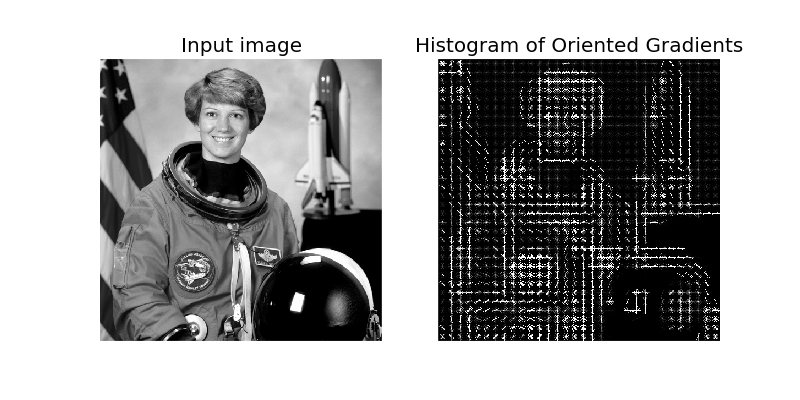
\includegraphics[scale=0.5]{figures/Chapter4/HOG2.png}
\caption{Example of Histogram of Oriented Gradients \Mycite{HOG}}
\end{figure}



\subsubsection{Scale Invariant Feature Transform(SIFT)}
In Harris Corner detection,the features are rotation-invariant but not scale invariant.So, in \citet{SIFT} proposed an algorithm which extracts keypoints and compute its descriptors. There are mainly four steps involved in SIFT algorithm. 
\begin{enumerate}
\item Scale-space extrema detection: The first stage of computation searches over all scales and image locations. It is implemented efficiently by using a difference-of-Gaussian
function to identify potential interest points that are invariant to scale and orientation.
\begin{figure}[!hbtp]
\centering
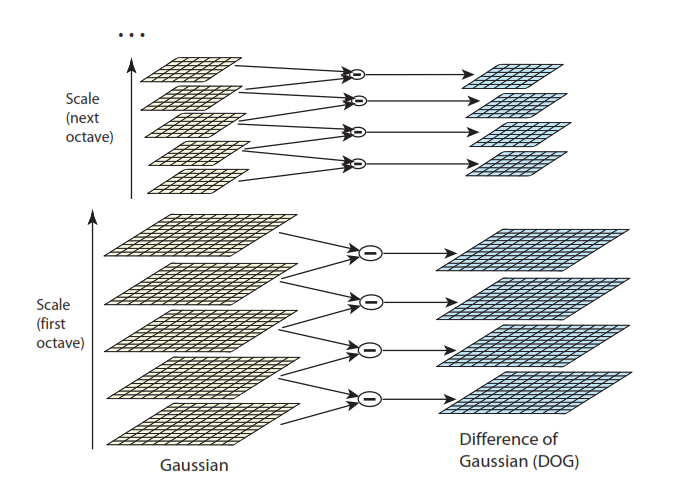
\includegraphics[scale=0.8]{figures/Chapter4/SIFT1.png}
\caption{Difference of Gaussians for SIFT \Mycite{SIFT}}
\end{figure}

\item Keypoint localization: At each candidate location, a detailed model is fit to determine location and scale. Keypoints are selected based on measures of their stability.

\item Orientation assignment: One or more orientations are assigned to each keypoint location based on local image gradient directions. All future operations are performed
on image data that has been transformed relative to the assigned orientation, scale, and
location for each feature, thereby providing invariance to these transformations.

\begin{figure}[!hbtp]
\centering
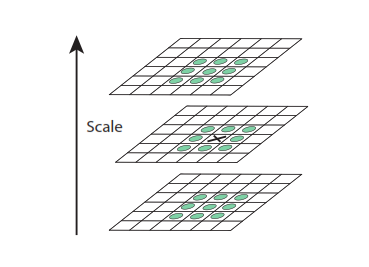
\includegraphics[scale=1]{figures/Chapter4/SIFT2.png}
\caption{Keypoint Localization in SIFT \Mycite{SIFT}}
\end{figure}

\item Keypoint descriptor: The local image gradients are measured at the selected scale
in the region around each keypoint. These are transformed into a representation that
allows for significant levels of local shape distortion and change in illumination
\end{enumerate}
\begin{figure}[!hbtp]
\centering
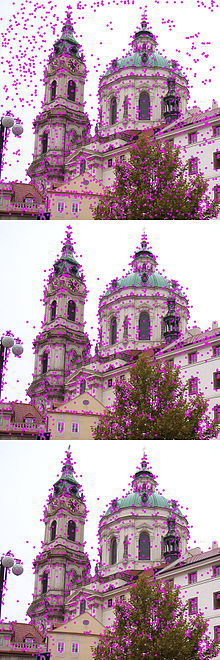
\includegraphics[scale=0.5]{figures/Chapter4/SIFT3.jpg}
\caption{Example of SIFT\Mycite{book_SIFT}}
\end{figure}
\newpage
\subsubsection{Speeded-Up Robust Features(SURF)}
In SIFT, Lowe approximated Laplacian of Gaussian with Difference of Gaussian for finding scale-space. SURF goes a little further and approximates LoG with Box Filter. One big advantage of this approximation is that, convolution with box filter can be easily calculated with the help of integral images. And it can be done in parallel for different scales. Also the SURF rely on determinant of Hessian matrix for both scale and location.\\
\begin{figure}[!hbtp]
\centering
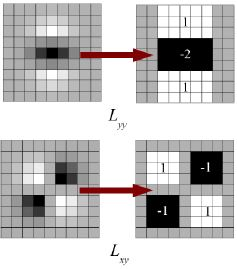
\includegraphics[scale=0.5]{figures/Chapter4/SURF1.jpg}
\caption{Approximation of LoG in SURF\Mycite{SURF}}
\end{figure}
\\
For orientation assignment, SURF uses wavelet responses in horizontal and vertical direction for a neighborhood of size 6s. Adequate Guassian weights are also applied to it.  The dominant orientation is estimated by calculating the sum of all responses within a sliding orientation window of angle 60 degrees. Interesting thing is that, wavelet response can be found out using integral images very easily at any scale. For many applications, rotation invariance is not required, so no need of finding this orientation, which speeds up the process. SURF provides such a functionality called Upright-SURF or U-SURF. It improves speed and is robust upto $\pm 15^{\circ}$.If it is 0, orientation is calculated. If it is 1, orientation is not calculated and it is more faster.
\begin{figure}[!hbtp]
\centering
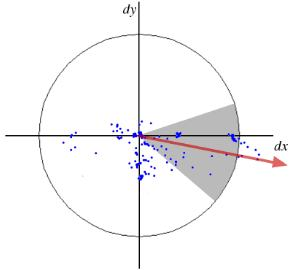
\includegraphics[scale=0.5]{figures/Chapter4/SURF2.jpg}
\caption{Plotting of wavelet responses in SURF\Mycite{SURF}}
\end{figure}\\
For feature description, SURF uses Wavelet responses in horizontal and vertical direction (again, use of integral images makes things easier). A neighbourhood of size 20sX20s is taken around the keypoint where s is the size. It is divided into 4x4 subregions. For each subregion, horizontal and vertical wavelet responses are taken and a vector is formed like this, v=$( \sum{d_x}, \sum{d_y}, \sum{|d_x|}, \sum{|d_y|})$. This when represented as a vector gives SURF feature descriptor with total 64 dimensions. Lower the dimension, higher the speed of computation and matching, but provide better distinctiveness of features.

For more distinctiveness, SURF feature descriptor has an extended 128 dimension version. The sums of $d_x$ and $|d_x|$ are computed separately for $d_y < 0$ and $d_y \geq 0$. Similarly, the sums of $d_y$ and $|d_y|$ are split up according to the sign of $d_x$ , thereby doubling the number of features. It doesn’t add much computation complexity. 

Another important improvement is the use of sign of Laplacian (trace of Hessian Matrix) for underlying interest point. It adds no computation cost since it is already computed during detection. The sign of the Laplacian distinguishes bright blobs on dark backgrounds from the reverse situation. In the matching stage, we only compare features if they have the same type of contrast. This minimal information allows for faster matching, without reducing the descriptor’s performance.\\
\begin{figure}[!hbtp]
\centering
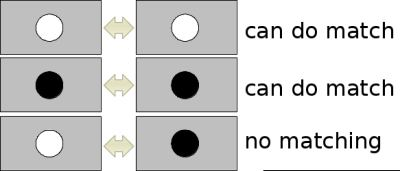
\includegraphics[scale=0.5]{figures/Chapter4/SURF3.jpg}
\caption{Comparing of features in SURF\Mycite{SURF}}
\end{figure}




\subsection{Motion Based Features}

\subsubsection{Space Time Interest Points(STIP)}
To detect spatio-temporal events, STIP builds on the idea of the Harris and Forstner interest point operators and detects local structures in space-time where the image values have significant local variations in both space and time.Then, the spatio-temporal extents of the detected events are estimated and their scale-invariant spatio-temporal descriptors are computed.Using such descriptors, they classify events and construct video representation in terms of labeled space-time points.\Mycite{STIP}In this case:

\begin{itemize}
\item Videos are considered as volumes of pixels.
\item Spatio-temporal features are located at spatio-temporal salient points that are extracted with interest point operators.
\item Interest point structures are searched for that are stable under  rotation, viewpoint, scale and illumination changes.
\end{itemize} 

So, space time interest point detectors are extensions of 2D interest point detectors that incorporate temporal information.They are based on the detection of spatio-temporal corners which are located in region that exhibits a high variation of image intensity in all
three directions $(x, y,t)$. This requires that spatio-temporal corners are located at spatial corners such that they invert motion in two consecutive frames (high temporal gradient variation). They are identified from local maxima of a cornerness function computed for all pixels across spatial and temporal scales.
\\
\begin{figure}[!hbtp]
\centering
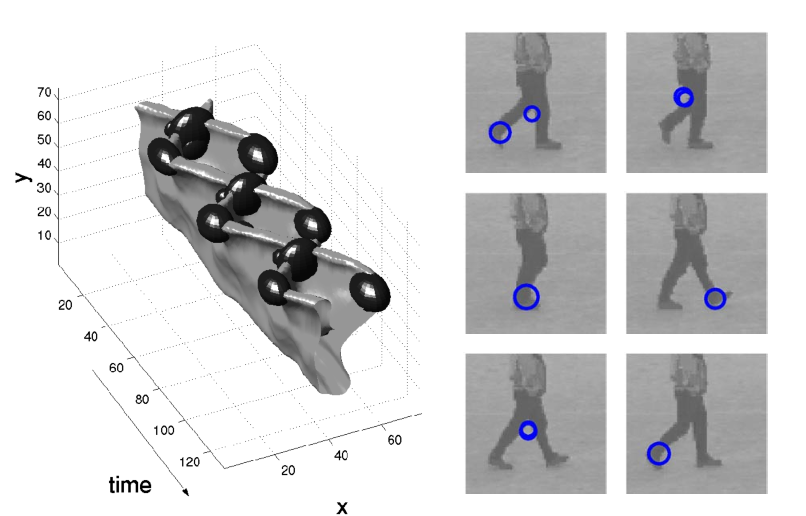
\includegraphics[scale=0.5]{figures/Chapter4/STIP.png}
\caption{Example of STIP \Mycite{STIP}}
\end{figure}
\\
\subsubsection{Optical Flow}
Optical flow is the pattern of apparent motion of image objects between two consecutive frames caused by the movement of object or camera. It is 2D vector field where each vector is a displacement vector showing the movement of points from first frame to second.\Mycite{Optical_flow}
Optical flow works on several assumptions:
\begin{itemize}
\item The pixel intensities of an object do not change between consecutive frames.
\item Neighboring pixels have similar motion. 
\end{itemize}
Consider a pixel $I(x,y,t)$ in first frame. It moves by distance $(dx,dy)$ in next frame taken after $dt$ time. So since those pixels are the same and intensity does not change, we can say,
\begin{equation}
I(x,y,t) = I(x+dx, y+dy, t+dt)
\end{equation}
Then take Taylor series approximation of right-hand side, remove common terms and divide by $dt$ to get the following equation:
\begin{equation}
f_x u + f_y v + f_t = 0 
\end{equation}
where
\begin{equation}
f_x = \frac{\partial f}{\partial x} \quad
f_y = \frac{\partial f}{\partial x} \quad
u = \frac{dx}{dt} \quad
v = \frac{dy}{dt}
\end{equation}
Above equation is called Optical Flow equation. In it, we can find $f_x$ and $f_y$, they are image gradients. Similarly $f_t$ is the gradient along time. But $(u,v)$ is unknown. We cannot solve this one equation with two unknown variables. So several methods are provided to solve this problem and one of them is Lucas-Kanade.

\textbf{Lucas Kanade method}-\\
We have seen an assumption before, that all the neighboring pixels will have similar motion. Lucas-Kanade method takes a $3x3$ patch around the point. So all the 9 points have the same motion. We can find $(f_x, f_y, f_t)$ for these 9 points. So now our problem becomes solving 9 equations with two unknown variables which is over-determined. A better solution is obtained with least square fit method. Below is the final solution which is two equation-two unknown problem and solve to get the solution.
\begin{equation}
\begin{bmatrix} u \\ v \end{bmatrix} =
\begin{bmatrix}
    \sum_{i}{f_{x_i}}^2  &  \sum_{i}{f_{x_i} f_{y_i} } \\
    \sum_{i}{f_{x_i} f_{y_i}} & \sum_{i}{f_{y_i}}^2
\end{bmatrix}^{-1}
\begin{bmatrix}
    - \sum_{i}{f_{x_i} f_{t_i}} \\
    - \sum_{i}{f_{y_i} f_{t_i}}
\end{bmatrix}
\end{equation}
So from user point of view, idea is simple, we give some points to track, we receive the optical flow vectors of those points. But again there are some problems. Until now, we were dealing with small motions. So it fails when there is large motion. So again we go for pyramids. When we go up in the pyramid, small motions are removed and large motions becomes small motions. So applying Lucas-Kanade there, we get optical flow along with the scale.

\subsubsection{Improved Trajectories}
These extracted trajectories are mainly located at regions with high motion salience, which contain rich and discriminative information. These local descriptors of the corresponding regions in several successive frames, are aligned and pooled along the trajectories. This trajectory constrained sampling strategy also takes account of the temporal continuity of human action, and is effective to deal with the variations of motion speed. However, these hand-crafted descriptors are not optimized for visual representation and may lack discriminative capacity for action recognition. To compute dense trajectories, 
\begin{enumerate}
\item  Densely sample a set of points on 8 spatial scales on a grid with step size of 5 pixels. Points in homogeneous areas are eliminated by setting a threshold for the smaller eigenvalue of their auto-correlation matrices. Then these sampled points
are tracked by media filtering of dense flow field.
\item The static trajectories are removed as they lack motion information, and other trajectories with suddenly large displacement are also ignored, since they are obviously incorrect due to inaccurate optical flow.
\end{enumerate}

\subsection{Audio Features}
Audio features can lead to three layers of audio understanding\Mycite{Survey} : Low-level acoustics, such as the average frequency for a frame, Mid-level sound objects, such as the audio signature of the sound a ball makes while bouncing, and High-level scene classes, such as background music playing in certain types of video scenes.

Audio features can be derived from either the time domain or the frequency domain. 
\begin{enumerate}
\item Time Domain Features-\\
The root mean square (RMS) of the signal energy approximates the human perception of
the loudness or volume of a sound .

\begin{itemize}
\item Zero crossing rate (ZCR) is the number of signal amplitude sign changes in the current frame. Higher frequencies result in higher zero crossing rates. Speech normally has a higher variability of the ZCR than in music. If the loudness and ZCR are both below thresholds, then this frame may represent silence.
\item The silence ratio is the proportion of a frame with amplitude values below some threshold. Speech normally has a higher silence ratio than music. 
\end{itemize}

\item Frequency Domain Features-\\
The energy distribution is the signal distribution across frequency components. 
\begin{itemize}
\item Brightness is approximated by the frequency centroid, provides a measure of where the frequency components are concentrated. Brightness is higher for music than speech.
\item Bandwidth is the measure of frequency range of the signal.
\item The fundamental frequency is the lowest frequency in a sample and approximates pitch, which is a subjective measure.
\item Mel-frequency cepstral coefficients (MFCC) are produced by taking the logarithm of the spectral components and then placing them into bins based upon the Mel frequency scale,
which is perception-based. This is followed by applying the discrete cosine transform (DCT)

\end{itemize}
\end{enumerate}


\section{Feature Encoding Methods}
There are 2 feature encoding methods when we consider a holistic approach:-
\begin{enumerate}
	\item Bag of Features - It is a standard approach in which we quantize the features into a predefined codebook.It is an orderless document representation methodology in which we compute the feature descriptors , then cluster them to get a frequency representation by use of hard clustering like KNN clustering. The mechanism is shown in Figure \ref{Bow}.
		
	\begin{figure}[hbtp]
	\centering
	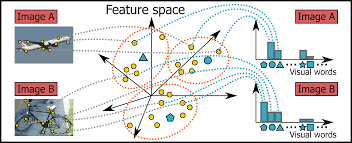
\includegraphics[scale=0.5]{figures/Feature_extraction/BoW.png}
	\caption{Bag of words representation}
	\label{Bow}
	\end{figure}
	
	\item Fisher Vectors - It encodes the second order feature information into an estimated Gaussian Mixture Model. The feature descriptors are represented by creating a GMM over the data and then providing soft labels to the data points. The mechanism is shown in Figure \ref{FV}.
	
	\begin{figure}[hbtp]
	\centering
	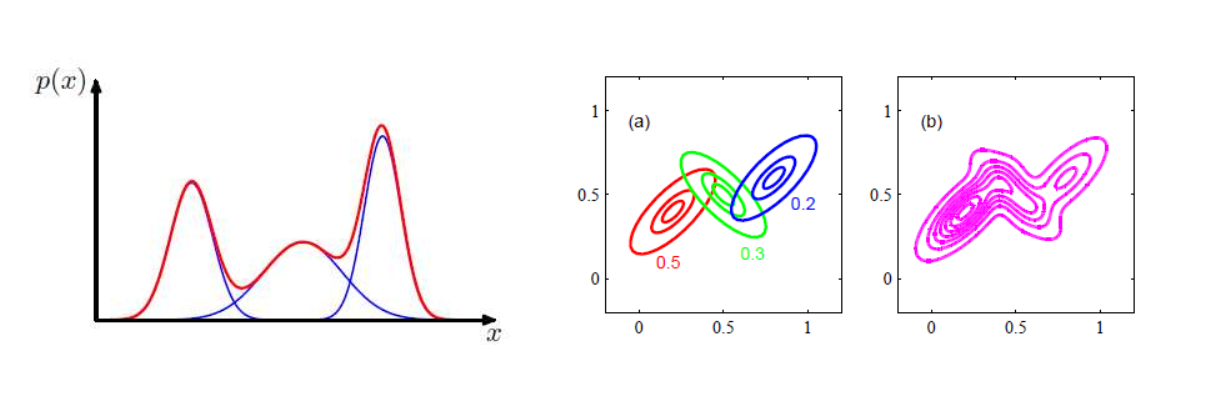
\includegraphics[scale=0.5]{figures/Feature_extraction/FV.png}
	\caption{Bag of words representation}
	\label{FV}
	\end{figure}
	
\end{enumerate}

\section{Summary}
In this chapter we studied about the various feature descriptors that can be used
for videos. We also studied the feature encoding methods and how they are evaluated. In the next chapter, we will look at the various classifiers that we can use dor the purpose of classifying videos.
